%\vspace{\sectionReduceTop}
\section{VQA Challenge and Workshop}
\label{sec:challenge}
%\vspace{\sectionReduceBot}

%We have collected questions for \textcolor{red}{200k} MS COCO images. \aishwarya{Do we still need to keep next line?} However, to increase the diversity of the dataset, we are also considering the addition of images from other sources. The use of more complex and diverse abstract scenes could also open up new application areas.
We have set up an evaluation server\footnote{\url{http://visualqa.org/challenge.html}} where results may be uploaded for the test set and it returns an accuracy breakdown. We are organizing an annual challenge and workshop to facilitate systematic progress in this area; the first instance of the workshop will be held at CVPR 2016\footnote{\url{http://www.visualqa.org/workshop.html}}. We suggest that papers reporting results on the VQA dataset --

\begin{compactenum}

\item Report test-standard accuracies, which can be calculated using either of the non-test-dev phases, i.e., ``test2015'' or ``Challenge test2015'' on the following links: [\href{https://www.codalab.org/competitions/6961}{oe-real} $|$ \href{https://www.codalab.org/competitions/6981}{oe-abstract} $|$ \href{https://www.codalab.org/competitions/6971}{mc-real} $|$ \href{https://www.codalab.org/competitions/6991}{mc-abstract}].

\item Compare their test-standard accuracies with those on the corresponding test2015 leaderboards [\href{http://www.visualqa.org/roe.html}{oe-real-leaderboard} $|$ \href{http://www.visualqa.org/aoe.html}{oe-abstract-leaderboard} $|$ \href{http://www.visualqa.org/rmc.html}{mc-real-leaderboard} $|$ \href{http://www.visualqa.org/amc.html}{mc-abstract-leaderboard}].
%\item Compare their test-standard accuracies with those on the corresponding test2015 leaderboards [\href{https://competitions.codalab.org/competitions/6961\#results}{oe-real-leaderboard} $|$ \href{https://www.codalab.org/competitions/6981\#results}{oe-abstract-leaderboard} $|$ \href{https://www.codalab.org/competitions/6971\#results}{mc-real-leaderboard} $|$ \href{https://www.codalab.org/competitions/6991\#results}{mc-abstract-leaderboard}]. 
%We are working on building a COCO-style leaderboard which can provide you with appropriate references to cite, but in the meantime, please use the information (such as username, teamname, \etc) from the test2015 leaderboards to refer to other entries.

\end{compactenum}

For more details, please see the challenge page\footnote{\url{http://visualqa.org/challenge.html}}. Screenshots of leaderboards for open-ended-real and multiple-choice-real are shown in \figref{fig:leaderboard-oe}.
% \figref{fig:leaderboard-real-oe} and \figref{fig:leaderboard-real-mc} respectively.
We also compare the test-standard accuracies of our best model (deeper LSTM Q + norm I) for both open-ended and multiple-choice tasks (real images) with other entries (as of \today) on the corresponding leaderboards in \tableref{tab:comparison_leaderboard}.

\begin{table}[t] \scriptsize
\setlength{\tabcolsep}{1.8pt}
\begin{center}
\begin{tabular}{@{} l  c  c  c  c  c  c c c@{}}
%\hline
\toprule
& \multicolumn{4}{c}{Open-Ended} & \multicolumn{4}{c}{ Multiple-Choice} \\

\cmidrule[0.75pt](l){2-5}
\cmidrule[0.75pt](l){6-9}
 & All & Yes/No & Number & Other & All & Yes/No & Number & Other \\
%\hline
\midrule
snubi-naverlabs & 60.60 & 82.23 & 38.22 & 46.99 
& 64.95 & 82.25 & 39.56 & 55.68 \\
MM\_PaloAlto & 60.36 & 80.43 & 36.82 & 48.33 
& -- & -- & -- & -- \\
LV-NUS & 59.54 & 81.34 & 35.67 & 46.10 
& 64.18 & 81.25 & 38.30 & 55.20 \\
ACVT\_Adelaide & 59.44 & 81.07 & 37.12 & 45.83 
& -- & -- & -- & --\\
global\_vision & 58.43 & 78.24 & 36.27 & 46.32 
& -- & -- & -- & --\\
deeper LSTM Q + norm I & 58.16 & 80.56 & 36.53 & 43.73 
& 63.09 & 80.59 & 37.70 & 53.64\\
iBOWIMG	 & -- & -- & -- & --
& 61.97 & 76.86 & 37.30 & 54.60\\
\bottomrule
\end{tabular}	
\caption{Test-standard accuracy of our best model (deeper LSTM Q + norm I) compared to test-standard accuracies of other entries for the open-ended and multiple-choice tasks in the respective VQA Real Image Challenge leaderboards (as of \today).}
%\vspace{-5pt}
\label{tab:comparison_leaderboard}
\end{center}
\end{table}

\begin{figure*}[h]
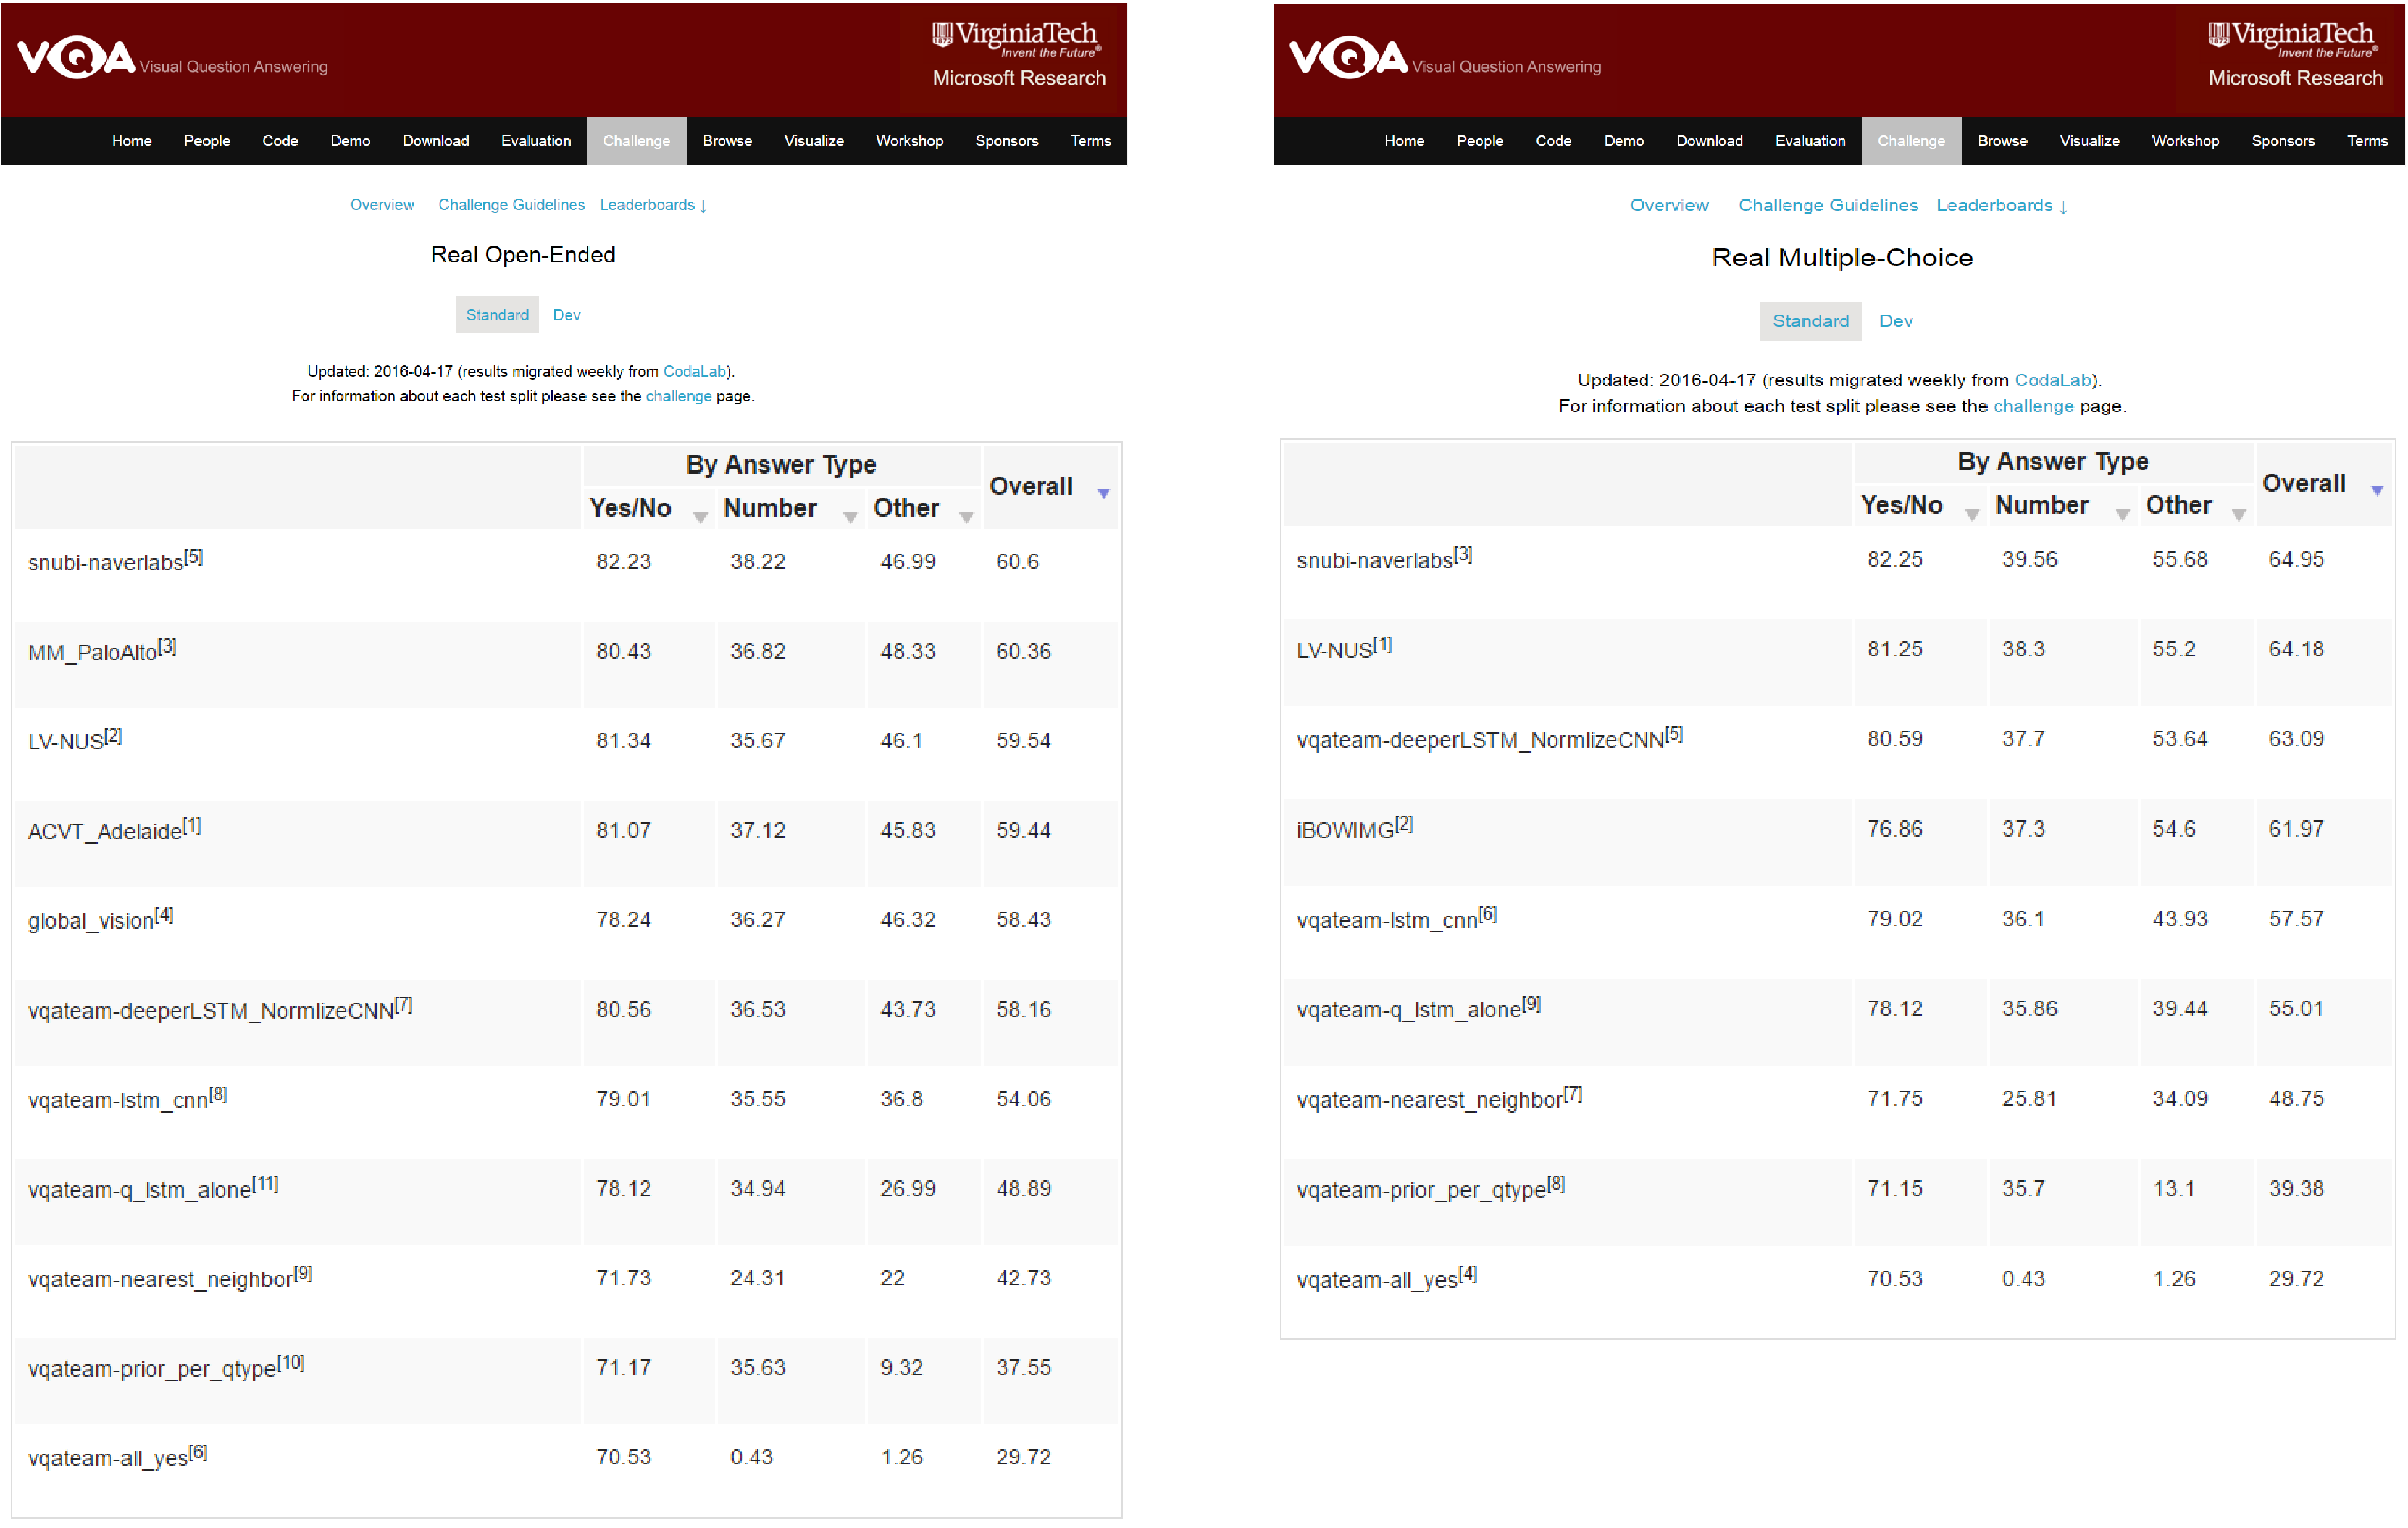
\includegraphics[width=1\linewidth]{figures/real-screenshot.pdf}
\centering
\caption{Leaderboard showing test-standard accuracies for VQA Real Image Challenge (Open-Ended) on left and leaderboard showing test-standard accuracies for VQA Real Image Challenge (Multiple-Choice) on right (snapshot from \today).}
\label{fig:leaderboard-oe}
%\vspace{\captionReduceBot}
\end{figure*}

%\begin{figure}[h!]
%\includegraphics[width=1\linewidth]{figures/real-oe-screenshot.pdf}
%\centering
%\caption{Leaderboard showing test-standard accuracies for VQA Real Image Challenge (Open-Ended) (snapshot from \today).}
%\label{fig:leaderboard-real-oe}
%%\vspace{\captionReduceBot}
%\end{figure}
%\begin{figure}[h!]
%\includegraphics[width=1\linewidth]{figures/real-mc-screenshot.pdf}
%\centering
%\caption{Leaderboard showing test-standard accuracies for VQA Real Image Challenge (Multiple-Choice) (snapshot from \today).}
%\label{fig:leaderboard-real-mc}
%%\vspace{\captionReduceBot}
%\end{figure} 